% Options for packages loaded elsewhere
\PassOptionsToPackage{unicode}{hyperref}
\PassOptionsToPackage{hyphens}{url}
%
\documentclass[
  english,
  man,floatsintext]{apa6}
\usepackage{lmodern}
\usepackage{amssymb,amsmath}
\usepackage{ifxetex,ifluatex}
\ifnum 0\ifxetex 1\fi\ifluatex 1\fi=0 % if pdftex
  \usepackage[T1]{fontenc}
  \usepackage[utf8]{inputenc}
  \usepackage{textcomp} % provide euro and other symbols
\else % if luatex or xetex
  \usepackage{unicode-math}
  \defaultfontfeatures{Scale=MatchLowercase}
  \defaultfontfeatures[\rmfamily]{Ligatures=TeX,Scale=1}
\fi
% Use upquote if available, for straight quotes in verbatim environments
\IfFileExists{upquote.sty}{\usepackage{upquote}}{}
\IfFileExists{microtype.sty}{% use microtype if available
  \usepackage[]{microtype}
  \UseMicrotypeSet[protrusion]{basicmath} % disable protrusion for tt fonts
}{}
\makeatletter
\@ifundefined{KOMAClassName}{% if non-KOMA class
  \IfFileExists{parskip.sty}{%
    \usepackage{parskip}
  }{% else
    \setlength{\parindent}{0pt}
    \setlength{\parskip}{6pt plus 2pt minus 1pt}}
}{% if KOMA class
  \KOMAoptions{parskip=half}}
\makeatother
\usepackage{xcolor}
\IfFileExists{xurl.sty}{\usepackage{xurl}}{} % add URL line breaks if available
\IfFileExists{bookmark.sty}{\usepackage{bookmark}}{\usepackage{hyperref}}
\hypersetup{
  pdftitle={Reminder about Confidence Intervals},
  pdfauthor={Marie Delacre1},
  pdfkeywords={keywords},
  hidelinks,
  pdfcreator={LaTeX via pandoc}}
\urlstyle{same} % disable monospaced font for URLs
\usepackage{graphicx,grffile}
\makeatletter
\def\maxwidth{\ifdim\Gin@nat@width>\linewidth\linewidth\else\Gin@nat@width\fi}
\def\maxheight{\ifdim\Gin@nat@height>\textheight\textheight\else\Gin@nat@height\fi}
\makeatother
% Scale images if necessary, so that they will not overflow the page
% margins by default, and it is still possible to overwrite the defaults
% using explicit options in \includegraphics[width, height, ...]{}
\setkeys{Gin}{width=\maxwidth,height=\maxheight,keepaspectratio}
% Set default figure placement to htbp
\makeatletter
\def\fps@figure{htbp}
\makeatother
\setlength{\emergencystretch}{3em} % prevent overfull lines
\providecommand{\tightlist}{%
  \setlength{\itemsep}{0pt}\setlength{\parskip}{0pt}}
\setcounter{secnumdepth}{-\maxdimen} % remove section numbering
% Make \paragraph and \subparagraph free-standing
\ifx\paragraph\undefined\else
  \let\oldparagraph\paragraph
  \renewcommand{\paragraph}[1]{\oldparagraph{#1}\mbox{}}
\fi
\ifx\subparagraph\undefined\else
  \let\oldsubparagraph\subparagraph
  \renewcommand{\subparagraph}[1]{\oldsubparagraph{#1}\mbox{}}
\fi
% Manuscript styling
\usepackage{upgreek}
\captionsetup{font=singlespacing,justification=justified}

% Table formatting
\usepackage{longtable}
\usepackage{lscape}
% \usepackage[counterclockwise]{rotating}   % Landscape page setup for large tables
\usepackage{multirow}		% Table styling
\usepackage{tabularx}		% Control Column width
\usepackage[flushleft]{threeparttable}	% Allows for three part tables with a specified notes section
\usepackage{threeparttablex}            % Lets threeparttable work with longtable

% Create new environments so endfloat can handle them
% \newenvironment{ltable}
%   {\begin{landscape}\begin{center}\begin{threeparttable}}
%   {\end{threeparttable}\end{center}\end{landscape}}
\newenvironment{lltable}{\begin{landscape}\begin{center}\begin{ThreePartTable}}{\end{ThreePartTable}\end{center}\end{landscape}}

% Enables adjusting longtable caption width to table width
% Solution found at http://golatex.de/longtable-mit-caption-so-breit-wie-die-tabelle-t15767.html
\makeatletter
\newcommand\LastLTentrywidth{1em}
\newlength\longtablewidth
\setlength{\longtablewidth}{1in}
\newcommand{\getlongtablewidth}{\begingroup \ifcsname LT@\roman{LT@tables}\endcsname \global\longtablewidth=0pt \renewcommand{\LT@entry}[2]{\global\advance\longtablewidth by ##2\relax\gdef\LastLTentrywidth{##2}}\@nameuse{LT@\roman{LT@tables}} \fi \endgroup}

% \setlength{\parindent}{0.5in}
% \setlength{\parskip}{0pt plus 0pt minus 0pt}

% Overwrite redefinition of paragraph and subparagraph by the default LaTeX template
% See https://github.com/crsh/papaja/issues/292
\makeatletter
\renewcommand{\paragraph}{\@startsection{paragraph}{4}{\parindent}%
  {0\baselineskip \@plus 0.2ex \@minus 0.2ex}%
  {-1em}%
  {\normalfont\normalsize\bfseries\itshape\typesectitle}}

\renewcommand{\subparagraph}[1]{\@startsection{subparagraph}{5}{1em}%
  {0\baselineskip \@plus 0.2ex \@minus 0.2ex}%
  {-\z@\relax}%
  {\normalfont\normalsize\itshape\hspace{\parindent}{#1}\textit{\addperi}}{\relax}}
\makeatother

% \usepackage{etoolbox}
\makeatletter
\patchcmd{\HyOrg@maketitle}
  {\section{\normalfont\normalsize\abstractname}}
  {\section*{\normalfont\normalsize\abstractname}}
  {}{\typeout{Failed to patch abstract.}}
\patchcmd{\HyOrg@maketitle}
  {\section{\protect\normalfont{\@title}}}
  {\section*{\protect\normalfont{\@title}}}
  {}{\typeout{Failed to patch title.}}
\makeatother
\shorttitle{CI REMINDER}
\keywords{keywords\newline\indent Word count: X}
\usepackage{lineno}

\linenumbers
\usepackage{csquotes}
\ifxetex
  % Load polyglossia as late as possible: uses bidi with RTL langages (e.g. Hebrew, Arabic)
  \usepackage{polyglossia}
  \setmainlanguage[]{english}
\else
  \usepackage[shorthands=off,main=english]{babel}
\fi

\title{Reminder about Confidence Intervals}
\author{Marie Delacre\textsuperscript{1}}
\date{}


\authornote{

Correspondence concerning this article should be addressed to Marie Delacre, Postal address. E-mail: \href{mailto:marie.delacre@ulb.be}{\nolinkurl{marie.delacre@ulb.be}}

}

\affiliation{\vspace{0.5cm}\textsuperscript{1} ULB}

\begin{document}
\maketitle

\hypertarget{introduction-how-to-compute-a-confidence-interval-around-pmbmu_1-mu_2}{%
\subsubsection{\texorpdfstring{Introduction: How to compute a confidence interval around \(\pmb{\mu_1-\mu_2}\)}{Introduction: How to compute a confidence interval around \textbackslash pmb\{\textbackslash mu\_1-\textbackslash mu\_2\}}}\label{introduction-how-to-compute-a-confidence-interval-around-pmbmu_1-mu_2}}

Considering the link between confidence intervals and NHST approach, we can think of the confidence limits as the most extreme values of \(\mu_1-\mu_2\) that we could define as null hypothesis and that would not lead to rejecting the null hypothesis (Cumming \& Finch, 2001), that is to say, the values associated with a \emph{p}-value that exactly equals \(\frac{alpha}{2}\).

Under the assumption of iid normal distribution of residuals with equal population variances across groups, in order to test the null hypothesis that \(\mu_1-\mu_2= (\mu_1-\mu_2)_0\), we can compute the following quantity:
\begin{equation*} 
t_{Student}=\frac{(\bar{X_1}-\bar{X_2})-(\mu_1-\mu_2)_0}{SE}
\label{eq:tstudent}
\end{equation*}
with \(SE = \sigma_{pooled} \times \sqrt{\frac{1}{n_1}+\frac{1}{n_2}}\) and \(\sigma_{pooled} = \sqrt{\frac{(n_1-1) \times S^2_1+(n_2-1)\times S^2_2}{n_1+n_2-2}}\).

Under the null hypothesis, this quantity will follow a central \emph{t}-distribution with \(n_1+n_2-2\) degrees of freedom. \footnote{Distribution is central because under the null hypothesis, the quantity is a (supposed normal) centered variable, divided by SE, an independant variable closely related with the $\chi^2$. }. The central \emph{t}-distribution is always centered around \((\mu_1-\mu_2)_0\). For example, when we expect that \(\mu_1=\mu_2\) under the null hypothesis, the central \emph{t}-distribution is centered around 0, when we expect that \(\mu_1-\mu_2=3\) under the null hypothesis, the central \emph{t}-distribution is centered around 3.

Considering all these information we can define \((\mu_1-\mu_2)_L\), the lower limit of the confidence interval, such as \(\frac{(\bar{X_1}-\bar{X_2})-(\mu_1-\mu_2)_L}{SE}\) exactly equals the quantile (1-\(\frac{\alpha}{2}\)) of the central \emph{t}-distribution of the null hypothesis \(H_0: \mu_1 - \mu_2 = (\mu_1-\mu_2)_L\) (i.e.~the symmetric \emph{t}-distribution that is centered around \((\mu_1-\mu_2)_L\)) and the upper limit \((\mu_1-\mu_2)_U\) such as \(\frac{(\bar{X_1}-\bar{X_2})-(\mu_1-\mu_2)_U}{SE}\) exactly equals the quantile \(\frac{\alpha}{2}\) of the central \emph{t}-distribution of the null hypothesis \(H_0: \mu_1 - \mu_2 = (\mu_1-\mu_2)_U\) (i.e.~the symmetric \emph{t}-distribution that is centered around \((\mu_1-\mu_2)_U\)):
\begin{equation*} 
Pr[t_{n_1+n_2-2} \geq \frac{(\bar{X_1}-\bar{X_2})-(\mu_1-\mu_2)_L}{SE}]= \frac{\alpha}{2}
\label{eq:plausiblelimit1}
\end{equation*}
\begin{equation*} 
Pr[t_{n_1+n_2-2} \leq \frac{(\bar{X_1}-\bar{X_2})-(\mu_1-\mu_2)_U}{SE}]= \frac{\alpha}{2}
\label{eq:plausiblelimit2}
\end{equation*}
Under the assumption of iid normal distribution of residuals with unequal variances across groups, in order to test the null hypothesis that \(\mu_1-\mu_2= (\mu_1-\mu_2)_0\), we can compute the following quantity:
\begin{equation*} 
t_{Welch}=\frac{(\bar{X_1}-\bar{X_2})-(\mu_1-\mu_2)_0}{SE}
\label{eq:twelch}
\end{equation*}
with \(SE = \sqrt{\frac{S^2_1}{n_1}+\frac{S^2_2}{n_2}}\). Again, under the null hypothesis, we know that this quantity will follow a central \emph{t}-distribution with \(df=\frac{(\frac{S^2_1}{n_1}+\frac{S^2_2}{n_2})^2}{\frac{(\frac{S^2_1}{n_1})^2}{n_1-1}+\frac{(\frac{S^2_2}{n_2})^2}{n_2-1}}\) degrees of freedom. We can therefore easily define \((\mu_1-\mu_2)_L\) such as \(\frac{(\bar{X_1}-\bar{X_2})-(\mu_1-\mu_2)_L}{SE}\) exactly equals the quantile (1-\(\frac{\alpha}{2}\)) of the central \emph{t}-distribution of the null hypothesis \(H_0: \mu_1 - \mu_2 = (\mu_1-\mu_2)_L\), and the upper limit \((\mu_1-\mu_2)_U\) such as \(\frac{(\bar{X_1}-\bar{X_2})-(\mu_1-\mu_2)_U}{SE}\) exactly equals the quantile \(\frac{\alpha}{2}\) of the central \emph{t}-distribution of the null hypothesis \(H_0: \mu_1 - \mu_2 = (\mu_1-\mu_2)_U\):
\begin{equation*} 
Pr[t_{df} \geq \frac{(\bar{X_1}-\bar{X_2})-(\mu_1-\mu_2)_L}{SE}]= \frac{\alpha}{2}
\label{eq:plausiblelimit1}
\end{equation*}
\begin{equation*} 
Pr[t_{df} \leq \frac{(\bar{X_1}-\bar{X_2})-(\mu_1-\mu_2)_U}{SE}]= \frac{\alpha}{2}
\label{eq:plausiblelimit2}
\end{equation*}
It is not the most conventional way of computing confidence limits around any mean differences, however this approach is interesting as it helps to understand how to compute confidence limits around a measure of effect size.

\hypertarget{how-to-compute-a-confidence-interval-around-a-point-estimator}{%
\subsubsection{How to compute a confidence interval around a point estimator}\label{how-to-compute-a-confidence-interval-around-a-point-estimator}}

\begin{figure}
\centering
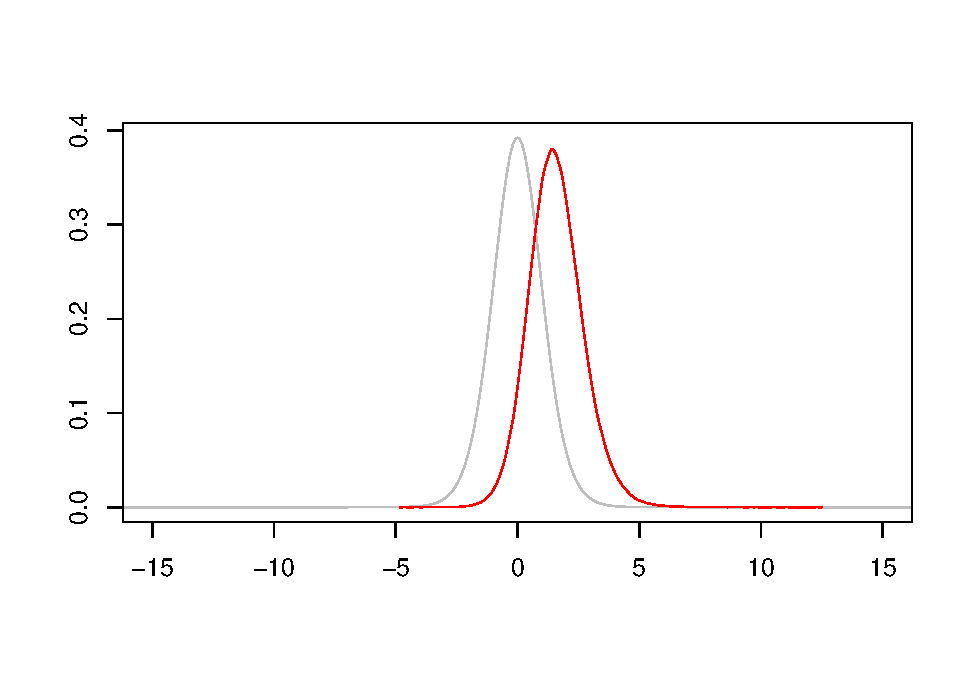
\includegraphics{CI_files/figure-latex/SAMPLMEANDIFF3-1.pdf}
\caption{\label{fig:SAMPLMEANDIFF3}Sampling distribution of centered mean difference divided by SE (in grey) and not centered mean difference divided by SE (in red), assuming normality and homoscedasticity.}
\end{figure}

As illustration, we will explain how to compute a confidence interval around Cohen's \(d_s\) (the explanation would be very similar for all other estimators). We previously mentioned that when the null hypothesis is true, \(t_{Student}\) follows a central \emph{t}-distribution. However, when the null hypothesis is false, the distribution of this quantity is not centered and noncentral \emph{t}-distribution arises (Cumming \& Finch, 2001), as illustrated in Figure \ref{fig:SAMPLMEANDIFF3}.

Noncentral \emph{t}-distributions are described by two parameters: degrees of freedom (\(df\)) and noncentrality parameter (that we will call \(\Delta\); Cumming \& Finch, 2001), the last being a function of \(\delta\) and sample sizes \(n_1\) and \(n_2\):
\begin{equation*}
\Delta = \frac{\mu_1-\mu_2}{\sigma_{pooled}} \times \sqrt{\frac{n_1 \times n_2}{n_1 + n_2}}
\label{eq:ncp}
\end{equation*}
Considering the link between \(\Delta\) and \(\delta\), it is possible to compute confidence limits for \(\Delta\) and divide them by \(\sqrt{\frac{n_1 \times n_2}{n_1 + n_2}}\) in order to have confidence limits for \(\delta\). In other words, we first need to determine the noncentrality parameters of the \emph{t}-distributions for which \(t_{Student}\) corresponds respectively to the quantiles \(\left(1-\frac{\alpha}{2}\right)\) and \(\frac{\alpha}{2}\):
\[P[t_{df, \Delta_L} \geq t_{Student}] = \frac{\alpha}{2} \]
\[P[t_{df, \Delta_U} \leq t_{Student}] = \frac{\alpha}{2} \]
with \(df = n_1+n_2-2\). Second, we divide \(\Delta_L\) and \(\Delta_U\) by \(\sqrt{\frac{n_1 \times n_2}{n_1 + n_2}}\) in order to define \(\delta_L\) and \(\delta_U\):
\[\delta_L = \frac{\Delta_L}{\sqrt{\frac{n_1 \times n_2}{n_1 + n_2}}}\]
\[\delta_U = \frac{\Delta_U}{\sqrt{\frac{n_1 \times n_2}{n_1 + n_2}}}\]

\hypertarget{refs}{}
\leavevmode\hypertarget{ref-Cumming_Finch_2001}{}%
Cumming, G., \& Finch, S. (2001). A primer on the understanding, use, and calculation of confidence intervals that are based on central and noncentral distributions. \emph{Educational and Psychological Measurement}, \emph{61}(532), 532--574.


\end{document}
